\section{Interface} % fold
\label{sub:interface}
  Para a realização da interface com o usuário, foi criado uma aplicação web, utilizando o \textit{framework} livre, Ruby on Rails\cite{rails}.
Esse \textit{framework} permite desenvolvimento de sites e usa como linguagem o Ruby. Sua arquitetura padrão é o MVC(\textit{Model-View-Controller}),
 que basicamente separa a aplicação em 3 camadas. A camada de interação do usuário(\textit{view}), a camada de manipulação dos dados(\textit{model}) 
e a camada de controle(\textit{controller})\cite{mvc}.
  O rails permite adicionar bibliotecas com funções especias, essas bibliotecas tem o nome de \textit{gem}. Para a aplicação, além das gems padrões, também serão utilizadas as gems descritas na tabela \ref{gems}.
\begin{table}[H]
\centering
\caption{Gems}
\label{gems}
\begin{tabular}{|l|l|}
\hline
\rowcolor[HTML]{C0C0C0} 
{\color[HTML]{333333} \textbf{Gem}} & {\color[HTML]{333333} \textbf{Descrição}} \\ \hline
devise\_ldap\_authenticatable       & Para autenticar junto com uma base LDAP   \\ \hline
cancancan                           & Para autorização                          \\ \hline
rolify                              & Para criar funções de usuários            \\ \hline
fullcalendar-rails                  & Para mostrar calendário de agendamento    \\ \hline
momentjs-rails                      & Auxílio ao calendário                     \\ \hline
bootstrap-sass                      & Para layout das páginas                   \\ \hline
rails-erd                           & Para gerar diagrama de classe             \\ \hline
\end{tabular}
\end{table}

A figura \ref{img:diagrama} mostra o diagrama de domínio do projeto

\begin{figure}[H]
	\centering
	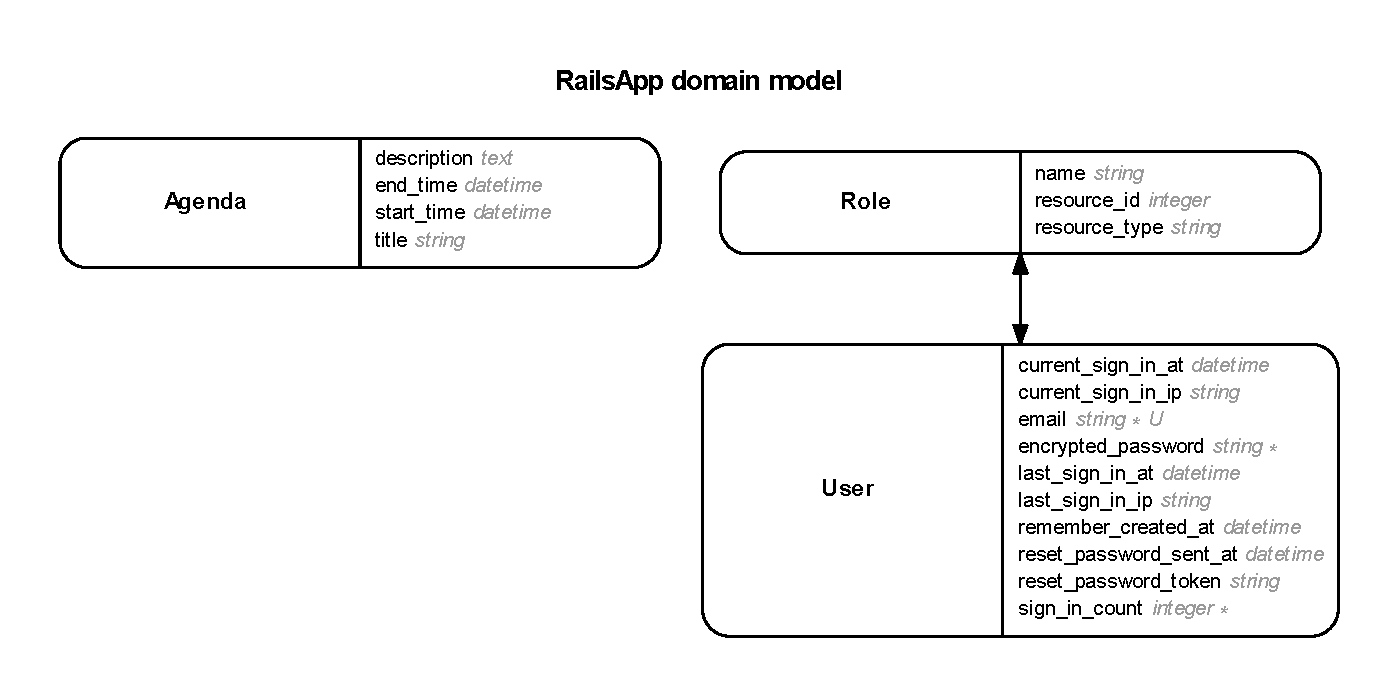
\includegraphics[scale=0.7]{figuras/erd.pdf}
	\caption{Diagrama de domínio.}
	\label{img:diagrama}
\end{figure}

A classe \textit{User} foi criada para realizar o login na aplicação, sendo utilizada em conjunto com a \textit{gem} devise\_ldap\_authenticable. Ela possui um relacionamento com a classe \textit{Role} que atribui uma função ao usuário. Atualmente, só está sendo utilizado a função de administrador. Por fim, a classe Agenda é responsável por guardar os agendamentos feitos pelo usuário. O código da interface do R2-PI2 está no \href{https://github.com/PI2Aspirador/railsApp}{Github}.

As imagens a seguir mostram como está a interface.

\begin{figure}[H]
	\centering
	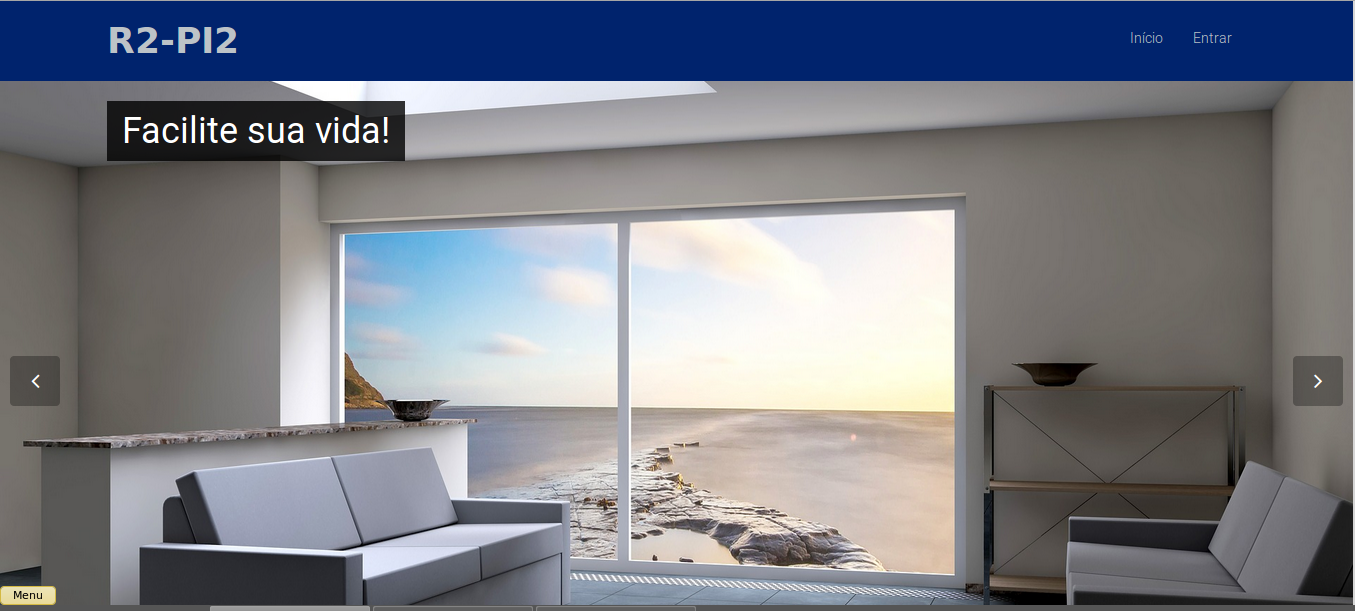
\includegraphics[scale=0.3]{figuras/home_interface.png}
	\caption{Interface - Home.}
	\label{img:home}
\end{figure}

\begin{figure}[H]
	\centering
	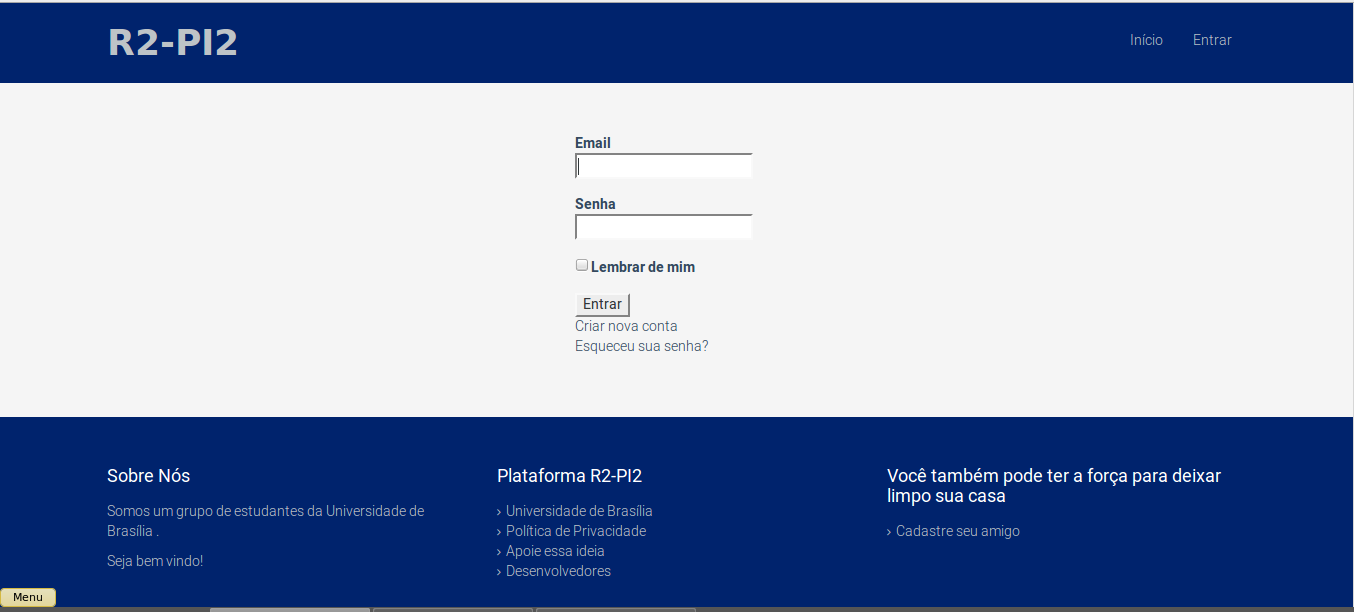
\includegraphics[scale=0.3]{figuras/login.png}
	\caption{Interface - Login.}
	\label{img:login}
\end{figure}

\begin{figure}[H]
	\centering
	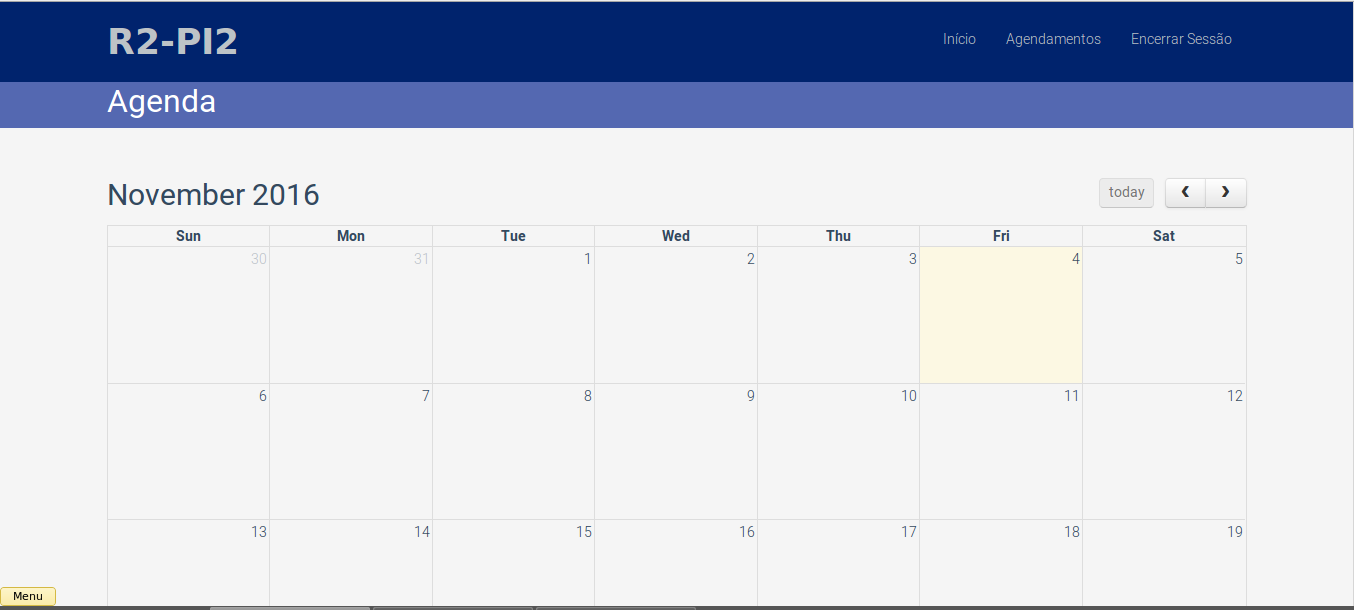
\includegraphics[scale=0.3]{figuras/agendamento.png}
	\caption{Interface - Agendamento.}
	\label{img:agendamento}
\end{figure}


\subsection{Validação experimental} % (fold)
	\label{sub:validação_experimental}

  Para a validação, não utilizamos nenhuma ferramenta que o rails possui devido a alteração constante da interface. Porém fizemos vários testes manuais,
 e por fim estabilizamos a interface do site, podendo ser acrescentado para a próxima entrega, uma ferramenta que auxilie e facilite tais testes.
